\chapter{通过 RNA-Seq 数据估计转录本的长度}
\label{chap-lenest}

\section{介绍}
在这里我们给出一个能够通过 RNA-Seq 数据在没有已知基因注释的情况下估计一个转录本的长度的统计方法。 

对于目前大部分现有的 RNA-Seq 数据, 
我们都无法直接从数据中直接获得其所包含的转录本在基因组上的 5' 段和 3' 段的位置。 
但是在 RNA-Seq 实验中为了能够测量每一个转录本的表达量, 
我们在计算其表达量时均需要使用到该转录本的长度 
\cite{mortazavi2008mapping, Jiang15042009, cufflinks.2010}。 
在使用基因组及其所对应的基因注释的情况下 (例如 RefSeq \cite{_refseq}), 
在分析时可以直接采用注释中的基因位置得出各转录本的长度。 
在没有基因注释, 或者在没有基因组参考序列的情况下, 
如果不采用更加复杂的技术, 如 RNA-PET \cite{Fullwood01042009} 技术, 
则需要通过 RNA-Seq 数据估计出转录本的长度。 对于现有的大部分 RNA-Seq 数据, 
仍然没有对应的 RNA-PET 数据用语确定各转录本的 5' 和 3' 段。 
所以对于通过 RNA-Seq 数据直接估计转录本的长度是有需求的。 

\section{理论分析}
在通过 RNA-Seq 数据估计转录本的时候我们对 RNA-Seq 数据做如下的假设以简化模型: 
\begin{itemize}
\item 所有的读段在原转录本上的位置的分布都是独立的 

\item 读段的 5' 段位置 (以下称之为起始位置) 在原转录本上的分布是均匀的。 
同样的, 读段的 3' 段位置 (以下称之为终止位置) 在原转录本上的分布也是均匀的 
\end{itemize}

此处为了方便我们的讨论, 我们还假设: 
\begin{itemize}
\item 所有的读段的长度都是相同的, 为 $R$ bp 长
\end{itemize}

为了在基因组参考序列没有基因注释, 甚至于没有基因组参考序列, 
的情况下能够通过 RNA-Seq 数据估计出转录本的长度, 
我们在这里给出定理 \ref{len-est-thm-one-end} 和 
定理 \ref{len-est-thm-2-ends} 及其证明。 
通过定理 \ref{len-est-thm-one-end} 和 
定理 \ref{len-est-thm-2-ends} 
我们可以通过 RNA-Seq 数据估计出转录本的长度。 

\nocite{casella2002statistical} 

\begin{thm}
\label{len-est-thm-one-end}
假设 $X_1$, $X_2$, \ldots, $X_N$ 是来自定义在 
${1, 2, \ldots , L}$, $L \in \mathbb{Z}^+$ 的均匀分布, 
即 
\[
P(X = i) =  \begin{cases}
\frac{1}{L} & \text{ 当 } 1 \leq i \leq L \\
0 & \text{ 其余情况 }
\end{cases}
\]
则对于 $L$ 的最小方差无偏估计 $\hat{L}$ 为
\begin{equation}
\label{len-est-thm-on-end-eq}
\hat{L} = \frac{ {X_{(N)}}^{N+1} - (X_{(N)} - 1)^{N+1} }{ {X_{(N)}}^N - (X_{(N)} - 1)^N }
\end{equation}
其中 $X_{(N)} = \max_{1 \leq i \leq N} X_i$。 
\end{thm}

通过定理 \ref{len-est-thm-one-end} 我们可以在已知转录本上一个固定的位点 
(例如外显子出现剪切现象的边界), 根据读段的起始位置 (或者终止位置), 
估计出着一个位于转录本上的固定的位点到转录本的一端的序列的长度, 
从而能够估计出转录本的长度。 

下面我们给出定理 \ref{len-est-thm-one-end} 的证明。 

\begin{proof}
我们首先说明 
\[
X_{(N)} = \max_{1 \leq i \leq N} X_i
\] 
在定理中的假设下是一个充分统计量。 

由于在这里考虑的是一个离散的均匀分布, 我们容易注意到
\[
P(X_1, X_2, \ldots, X_N | X_{(N)}) = \frac{1}{ {X_{(N)}}^N - (X_{(N)} - 1)^N }
\]
与该分布的参数 $L$无关, 所以 $X_{(N)}$ 是一个充分统计量。 

另外, 根据离散的均匀分布的性质我们可以得到
\[
P(X_{(N)} = i) = \frac{ i^N - (i - 1)^N }{L^N}
\]

对于定理 \ref{len-est-thm-one-end} 中给出的估计 $\hat{L}$ 
(式 \eqref{len-est-thm-on-end-eq}), 
我们可以进一步计算 $\operatorname{E}[\hat{L}]$ 得
\begin{align*}
\operatorname{E}[\hat{L}] &= \sum_{i=1}^L P(X_{(N)} = i) 
    \frac{i^{N+1} - (i-1)^{N+1}}{i^N-(i-1)^{N-1}} \\
&= L
\end{align*}
从而我们可以知道定理 \ref{len-est-thm-one-end} 中给出的估计 $\hat{L}$ 
(式 \eqref{len-est-thm-on-end-eq}) 是无偏的。 

下面我们说明 $X_{(N)}$ 是一个完全统计量。 
即对于所有的 $L \in \mathbb{Z}^+$, 若有一个函数 $g(x)$, $x \in \mathbb{Z}^+$ 使得
\[
\operatorname{E}[g(X_{(N)})] = 0
\]
则 $g(x) = 0$ 对所有 $x \in \mathbb{Z}^+$ 成立。 

注意到
\[
\operatorname{E}[g(X_{(N)})] = 0
\]
对所有的 $L \in \mathbb{Z}^+$ 成立意味着
\begin{align*}
\frac{1^N - 0^N}{1^N} g(1) &= 0 \\
\frac{1^N - 0^N}{2^N} g(1) + \frac{2^N - 1^N}{2^N} g(2) &= 0 \\
\frac{1^N - 0^N}{3^N} g(1) + \frac{2^N - 1^N}{3^N} g(2) + \frac{3^N - 2^N}{3^N} g(3) &= 0 \\
\ldots
\end{align*}
所以根据数学归纳法, 我们容易得出 $g(x) = 0$ 对所有 $x \in \mathbb{Z}^+$ 成立。 
进而我们可以知道 $X_{(N)}$ 是一个完全统计量。 

由以上的分析我们知道: 
\begin{itemize}
\item $X_{(N)}$ 是一个充分统计量
\item $X_{(N)}$ 是一个完全统计量
\item 定理 \ref{len-est-thm-one-end} 中给出的估计 $\hat{L}$ 
(式 \eqref{len-est-thm-on-end-eq}) 对于此处的分布的参数 $L$ 的估计是无偏的 
\end{itemize}
从而根据 Lehmann-Scheff{\'e} 定理
\cite{lehmann2012completeness.p1, lehmann2012completeness.p2} 
我们可以得出定理 \ref{len-est-thm-one-end} 中给出的估计 $\hat{L}$ 
(式 \eqref{len-est-thm-on-end-eq}) 是对该分布的参数 $L$ 的最小方差无偏估计。 

\end{proof}

\begin{thm}
\label{len-est-thm-2-ends}
假设$X_1$, $X_2$, \ldots, $X_N$ 是来自定义在 
${p+1, p+2, \ldots , p+L}$, $p \in \mathbb{Z}$, $L \in \mathbb{Z}^+$ 的均匀分布, 
即 
\[
P(X = i) =  \begin{cases}
\frac{1}{L} & \text{ 当 } p+1 \leq i \leq p+L \\
0 & \text{ 其余情况 }
\end{cases}
\]
则对于 $L$ 的一个无偏估计 $\hat{L}$ 为
\begin{equation}
\label{len-est-thm-2-ends-eq}
\hat{L} = \frac{ D^{N+1} - 2 (D-1)^{N+1} + (\max(D-2, 0))^{N+1} }{ D^{N} - 2 (D-1)^{N} + (\max(D-2, 0))^{N} }
\end{equation}
其中 $D = \max_{1 \leq i \leq N} X_i - \min_{1 \leq i \leq N} X_i +1$。 
\end{thm}

通过定理 \ref{len-est-thm-2-ends} 我们可以在转录本上无法找到一个固定的位点时, 
通过 RNA-Seq 数据对转录本的长度进行估计。 
这种情况适用于在一个基因没有出现选择性剪切的现象时估计该转录本的长度, 
例如真核生物中只有一个外显子的基因或者是原核生物中的单个操纵子。 

下面我们给出定理 \ref{len-est-thm-2-ends} 的证明。 

\begin{proof}
根据均匀分布的性质, 我们容易得到
\[
P(D=i) = (L-D +1) \frac{ D^N - 2 (D-1)^N  + (\max(D-2,0))^N}{ L^N }
\]
从而
\begin{align*}
\operatorname{E}[\hat{L}] &= \sum_{i=1}^L P(D=i) 
    \frac{i^{N+1}-2(i-1)^{N+1}+(\max(i-2,0))^{N+1}}{i^N-2(i-1)^N+(\max(i-2,0))^N} \\
&= \frac{1}{L^N} \sum_{i=1}^L (L-i+1)(i^{N+1}-2(i-1)^{N+1}+(\max(i-2,0))^{N+1}) \\
&= L
\end{align*}

\end{proof}

\subsection{无参考基因组序列的情况}
\nocite{ewens2005statistical} 

在没有参考基因组序列的情况下, 我们希望从拼装的所有连续段 (contig) 
中挑选出覆盖原先转录本部分较多 (例如该连续段是该转录本唯一的一个连续段) 的连续段。 
因为在没有参考基因组序列的情况下, 若要认为一个连续段代表原基因, 
则必须要求该连续段覆盖了原转录本的大部分的区域。 
如果一个转录本的测序深度偏低, 覆盖低, 
则通过测序的结果我们可能看到这个转录本会拥有多个连续段, 
这样的情况在没有参考序列时是几乎无法分析的。

下面我们给出我们对于选择 ``覆盖原转录本较多'' 的连续段的一种思路。

首先, 我们在这里介绍一个用来描述测序过程的 Poisson 模型 \cite{waterman1994sequence}。

我们定义测序的覆盖 (coverage) $c$
\begin{equation}
c = \frac{NR}{L}
\end{equation}
其中 $R$ 是测序读段的长度, $N$ 是转录本上测序时得到的读段的个数, 
$L$ 是转录本的有效长度 ($\text{转录本实际长度} -R+1$)。 

这里假设我们有一个无限长的序列, 
每一个位置上起始的读段个数都是一个参数为 $\lambda$ 的 Poisson 分布。 
并且所有位置的起始的读段个数均是独立的。 
在这里测序的覆盖和 $\lambda$ 的在理想的情况下满足如下的关系
\[
\lambda = c R
\]

当两个读段至少有一个碱基对重合时, 
我们认为这两个读段能够连接到一起组成一个更长的连续段。 通过这样的过程, 
我们将若干读段连接在一起构成连续段。 

为了挑选覆 ``覆盖原转录本较多'' 的连续段, 
我们在上面所述的测序模型下对每一个连续段考虑如下的一个概率
\begin{equation}
\label{lenest-one-contig-one-isof-prob-decription}
P(\text{观察到一个连续段其长度} \leq \text{目前的连续段 }\ |\text{ 目前的连续段的覆盖})
\end{equation}
这里的想法是, 如果对于一个给定的连续段, 
式 \eqref{lenest-one-contig-one-isof-prob-decription} 
中的概率较大, 则在这个连续段 ``变长'' 的过程中就已经 ``碰到了转录本的一端'' 无法 
``变得更长''。 

为了更深入地了解式 \eqref{lenest-one-contig-one-isof-prob-decription} 中的概率, 
我们在这里分析
\begin{equation}
\label{lenest-one-cont-prob-distr}
P(\text{连续段长度} = l\ | \text{目前的连续段的覆盖} \lambda)
\end{equation}
即给定覆盖, 连续段的长度的分布。 
下面为方便讨论我们记
\begin{equation}
p_n =  \frac{P(\text{连续段长度} = n+R-1 | \text{目前的连续段的覆盖} \lambda)}{e^{-(R-1)\lambda}}
\end{equation}
则
\begin{align}
p_n &= 0 & n &\leq 0 \\
p_1 &= 1 & & \\
p_{n+R} &= \sum_{i=1}^{R-1} (1-e^{-\lambda}) e^{-(R-1-i)\lambda} p_{n+i} & n &\geq 2-R
\end{align}

为了估计式 \eqref{lenest-one-contig-one-isof-prob-decription} 中的概率, 
在这里我们先介绍一个改进的 Lander-Waterman 公式 (定理 \ref{discrete-lander-waterman-thm}), 
原先的 Lander-Waterman 公式 \cite{lander1988genomic} 在推导中使用了一些近似, 
在这里我们不使用 Lander 和 Waterman 在 \onlinecite{lander1988genomic} 中所使用的近似。 

\begin{thm}[改进的 Lander-Waterman 公式]
\label{discrete-lander-waterman-thm}
在之前的 Poisson 模型下, 一个连续段的期望的长度
\begin{equation}
\label{discrete-lander-waterman-formula}
\operatorname{E}[\text{一个连续段的长度}] = \frac{e^{R\lambda} - 1}{e^\lambda - 1} 
\end{equation}
\end{thm}

下面我们给出定理 \ref{discrete-lander-waterman-thm} 的证明。 

\begin{proof}
这里为了描述的1简便, 我们记
\begin{align*}
q &= 1 - e^{-\lambda} \\
1-q &= e^{-\lambda}
\end{align*}

为了证明定理 \ref{discrete-lander-waterman-thm} 
中的式 \eqref{discrete-lander-waterman-formula}, 
我们考虑相邻的读段起始位置的个数 $N_D$ (即两个位置是相邻的两个读段起始位置, 
同时这两个位置上的读段连接在了一起), 
以及两个相邻的有读段的位置间的差值 $D_i$, $i=1,2,\ldots,N_D$ 
(即用 $X_1=1,X_2,\ldots,X_{N_D}, X_{N_D+1}$ 表示若干个相邻的读段起始位置时, 
$D_i=X_{i+1}-X_i$, $i=1,2,\ldots,N_D$)。 
根据这里所使用的模型, 我们容易知道 $D_i$, $i=1,2,\ldots,N_D$ 是 i.i.d.。 

所以我们容易看出来
\begin{align*}
\operatorname{E}[\text{一个连续段的长度}] &= \operatorname{E}[X_{N_D + 1}] +R-1 \\
&= \operatorname{E}[\sum_{i=1}^{N_D} D_i] +R \\
&= \operatorname{E}[\operatorname{E}[\sum_{i=1}^{N_D} D_i|N_D]] +R \\
&= \operatorname{E}[D] \operatorname{E}[N_D] +R
\end{align*}

下面我们分别计算
\begin{align*}
\operatorname{E}[D] \\
\operatorname{E}[N_D]
\end{align*}

根据这里所使用的模型, 我们可以知道
\[
P(D=i) \propto \begin{cases}
(1-q)^{i-1} q & i=1,2,\ldots,R-1 \\
0 & \text{其余情况}
\end{cases}
\]
所以可以计算得
\begin{align*}
\operatorname{E}[D] &= \frac{1}{1-(1-q)^{R-1}} \sum_{i=1}^{R-1} i (1-q)^{i-1} q \\
&= \frac{(q(R-1)+1)(1-q)^R-(1-q)}{-(1-q)q(1-(1-q)^{R-1})}
\end{align*}

同时, 我们根据模型可知
\[
P(N_D=j) = (1-q)^{R-1}(1-(1-q)^{R-1})^{j},\ j=0,1,\ldots
\]
根据几何分布的性质我们可知
\[
\operatorname{E}[N_D]=\frac{1-(1-q)^{R-1}}{(1-q)^{R-1}}
\]

综上所述, 进一步化简我们可得
\[
\operatorname{E}[D] \operatorname{E}[N_D] = \frac{e^{R\lambda} -1}{e^{\lambda}-1} -R
\]

故定理得证。 

\end{proof}

为了估计式 \eqref{lenest-one-contig-one-isof-prob-decription} 
中在给定覆盖 $\lambda$ 的情况下, 在无穷长的序列上观察到长度为 $l$ 的概率, 
我们将该分布近用一个期望是 $\operatorname{E}[\text{一个连续段的长度}] -R+1$ 的几何分布, 
从而估计出式 \ref{lenest-one-contig-one-isof-prob-decription} 
中在无穷长的序列上给定覆盖 $\lambda$ 观察到一个连续段其长度小于等于目前的连续段的概率
\begin{align}
\label{lenest-one-contig-one-isof-prob-est}
& P(\text{观察到一个连续段其长度} \leq \text{目前的连续段} l |\text{目前的连续段的覆盖} \lambda) \nonumber \\
\approx & \frac{l-R+1}{\frac{e^{R\lambda} -1}{e^{\lambda}-1} -R+1}
\end{align}

在有了式 \eqref{lenest-one-contig-one-isof-prob-est} 中的近似估计之后, 
我们可以在没有参考基因组序列的情况下挑选出来拼装结果中那些可能是大部分覆盖原转录本的那些连续段, 
对这些连续段的长度通过前面定理 \ref{len-est-thm-one-end} 和定理 
\ref{len-est-thm-2-ends} 中所述的方法进行估计, 
从而进一步估计得这些连续段所对应的转录本的表达量。 

%\section{仿真分析}

\section{实际 RNA-Seq 数据分析}
\label{len-est-real-rna-seq}

我们对来自 ENCODE \cite{encode} 的 RNA-Seq 数据 
\footnote{\url{http://hgdownload.cse.ucsc.edu/goldenPath/hg19/encodeDCC/wgEncodeCaltechRnaSeq/wgEncodeCaltechRnaSeqGm12878R1x75dAlignsRep2V2.bam}} 
进行了分析, 
用来在真实 RNA-Seq 数据上测试前面所叙述的估计转录本长度的方法。 
在分析中, 我们只对只有一个外显子的基因进行了分析。

图 \ref{real-len-VS-est-len} 给出了我们估计的转录本的长度和真实的转录本的长度的比较。
转录本实际长度和真实长度的 Pearson 相关系数 95\% 置信区间为 $[0.8749423, 0.8948220]$。 

图 \ref{len-ratio-VS-lambda} 给出了估计的转录本长度和真实的转录本长度之比 
($\frac{\text{估计的转录本长度}}{\text{真实的转录本长度}}$) 
和测序 $\lambda$ 
之间的关系。图 \ref{len-ratio-VS-lambda} 中无明显的关系。

\begin{figure}[!t]
\centering
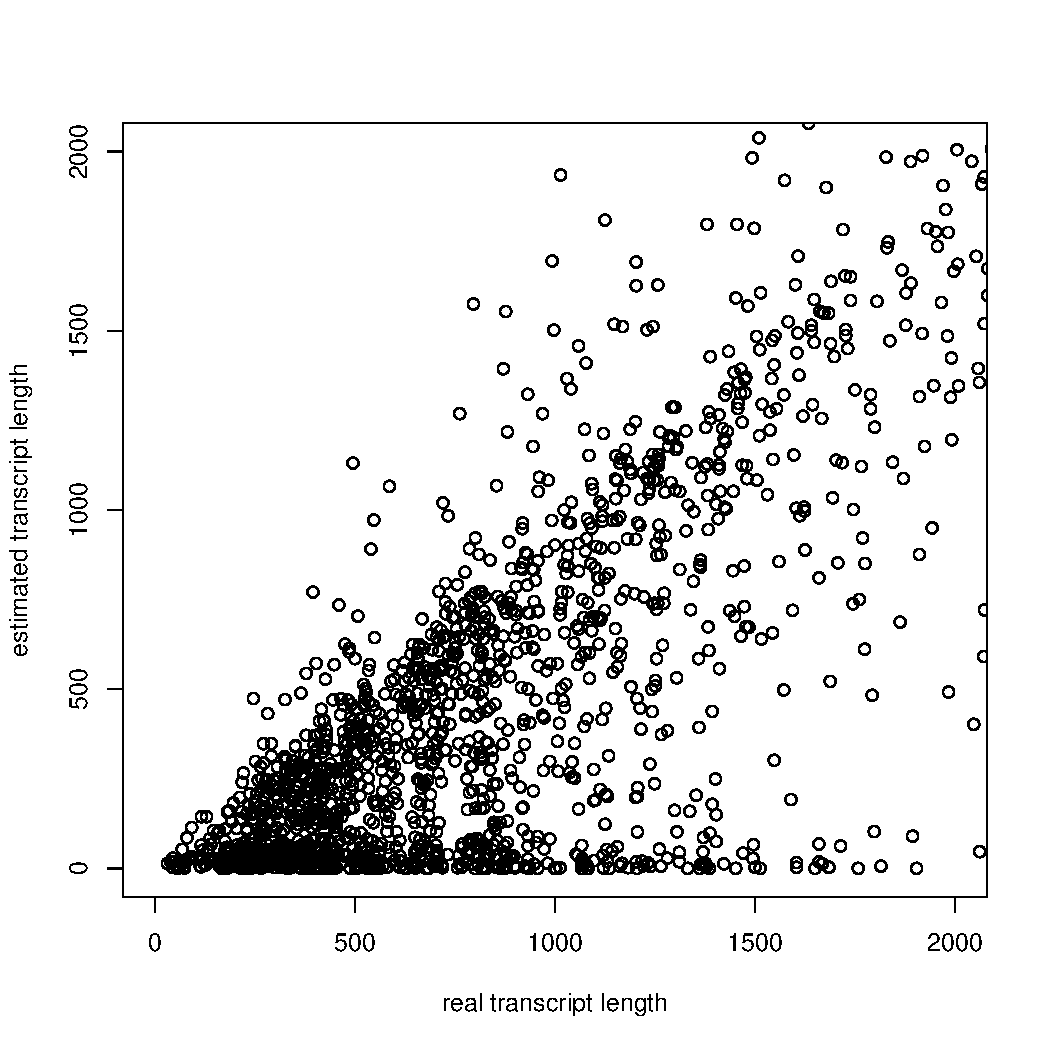
\includegraphics[width=\textwidth]{figures/lenest/real-len-VS-est-len.pdf}
\caption{实际的转录本长度和估计的转录本长度的比较}
\label{real-len-VS-est-len}
\end{figure}

\begin{figure}[!t]
\centering

    \begin{subfigure}{\textwidth}
        \centering
        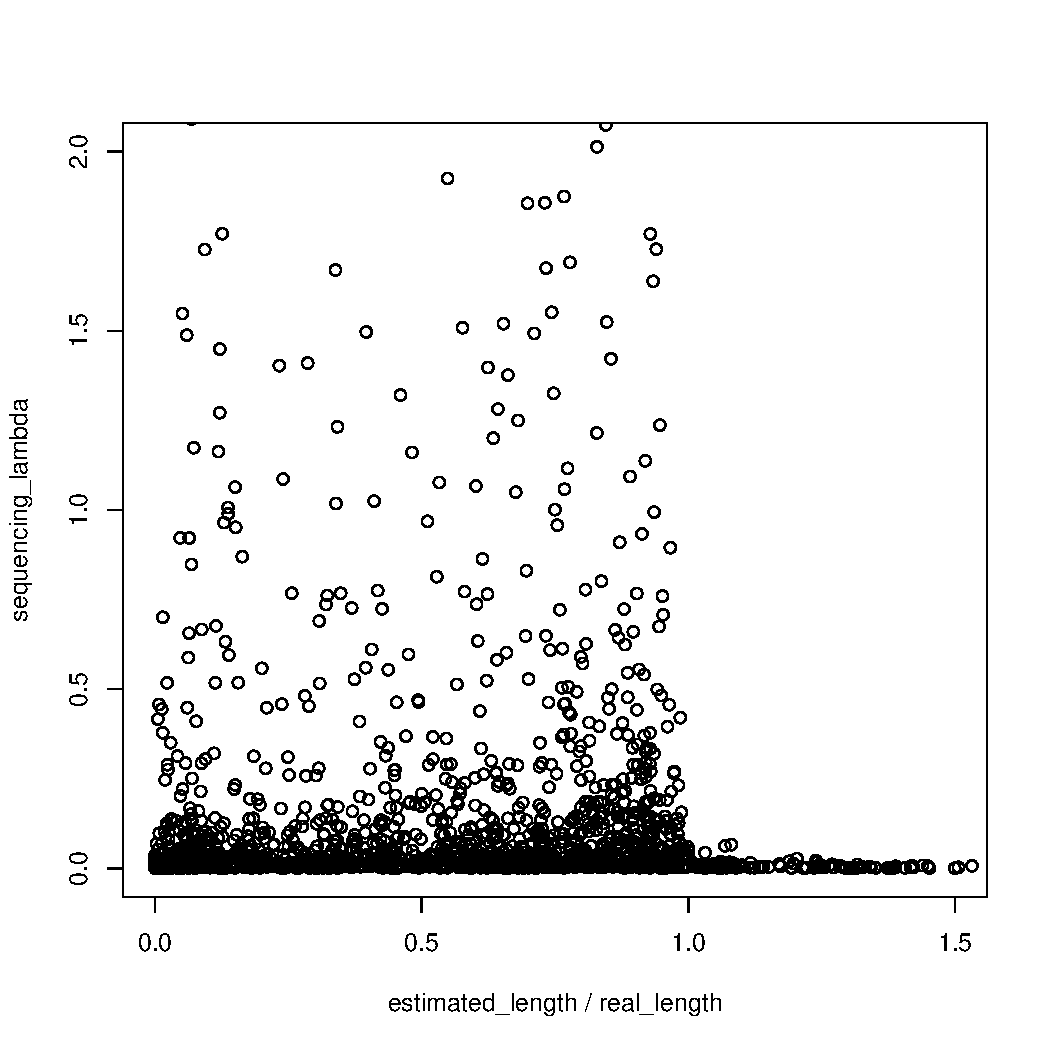
\includegraphics[width=0.45\textheight]{figures/lenest/lambda-len_ratio-2.pdf}
    \end{subfigure}
    
    \begin{subfigure}{\textwidth}
        \centering
        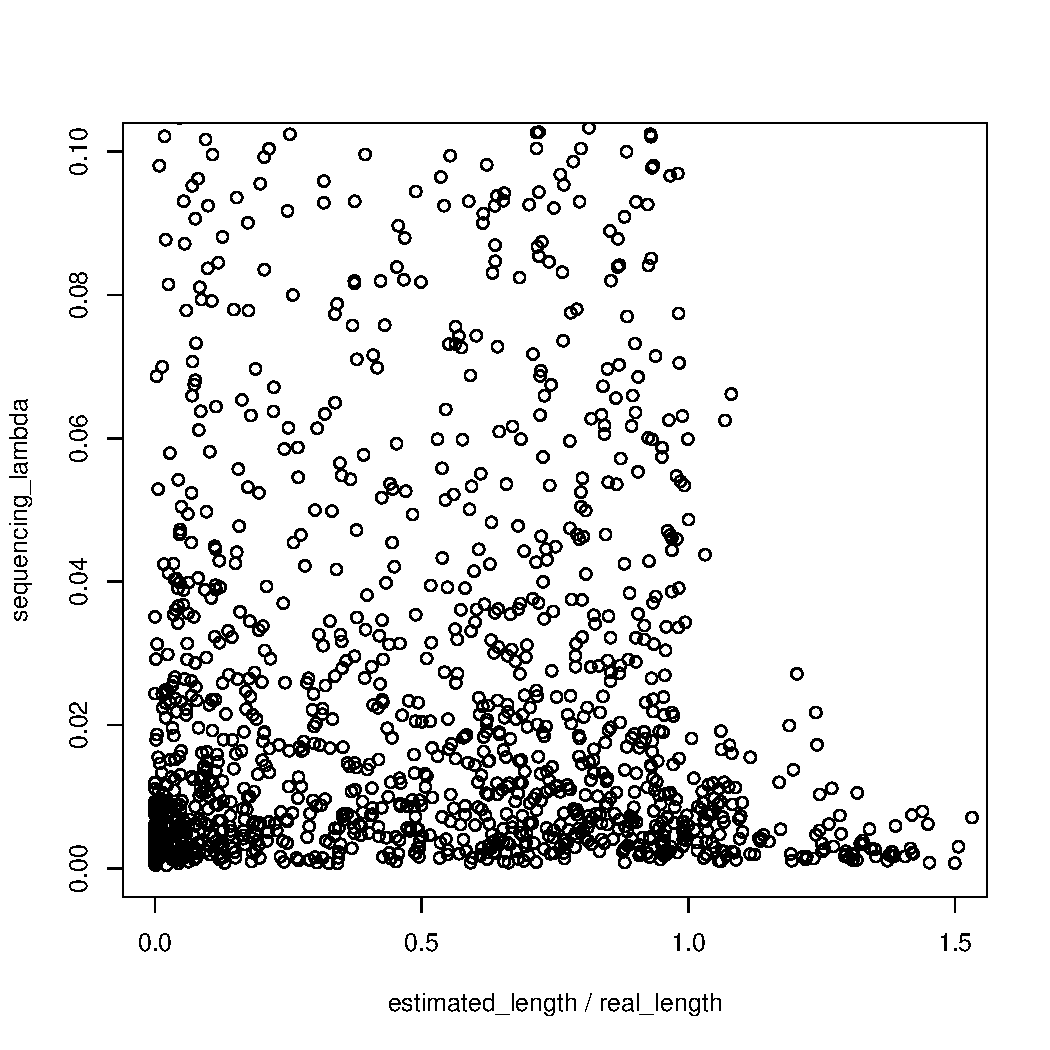
\includegraphics[width=0.45\textheight]{figures/lenest/lambda-len_ratio-0_10.pdf}
    \end{subfigure}


\caption{估计的转录本长度和真实的转录本长度之比 
($\frac{\text{估计的转录本长度}}{\text{真实的转录本长度}}$) 
和测序 $\lambda$ 
之间的关系}
\label{len-ratio-VS-lambda}
\end{figure}



